\section{Experiments}
\label{sec:exp}

In this section, we conduct extensive experiments to evaluate \prism, guided by the following questions: 
%(\textbf{RQ1}) Does the latent space of image models align well with fMRI signals? If not, which representation space shows stronger correspondence? 
(\textbf{RQ1}) How well does our framework \prism perform on the image reconstruction task? (\textbf{RQ2}) How do different choices of latent space influence the reconstruction quality? (\textbf{RQ3}) What is the contribution of each component in our framework to the overall reconstruction performance?

\subsection{Experimental Setup}
We conduct experiments on three datasets: NSD \citep{allen2022massive}, BOLD5000 \citep{chang2019bold5000}, and GOD \citep{horikawa2017generic}. Detailed descriptions of the datasets are provided in Section~\ref{app:dataset} of the Appendix. Each method is evaluated by comparing the reconstructed images to the ground truth using five metrics: PixCorr and SSIM for pixel- and structure-level similarity \citep{wang2004image}, LPIPS \citep{zhang2018unreasonable} for human perceptual similarity, and CLIP and Inception V3 two-way identification \citep{scotti2024mindeye2} for semantic consistency based on pretrained model representations.
%Pixelwise Correlation (PixCorr), Structural Similarity Index (SSIM) \citep{wang2004image}, Learned Perceptual Image Patch Similarity (LPIPS) \citep{zhang2018unreasonable}, which reflects human perceptual similarity, CLIP two-way identification (CLIP) \cite{scotti2024mindeye2} and Inception V3 two-way identification (Inception V3) \cite{scotti2024mindeye2}.
We compare our method against the following baselines: Takagi \& Nishimoto \citep{takagi2023high} (Takagi for short), Mindvis \citep{chen2023seeing}, Mindeye \citep{scotti2023reconstructing}, \textcolor{black}{MindBridge~\citep{wang2024mindbridge}, NeuralDiffuser~\citep{li2025neuraldiffuser}}, and Mindeye2 \citep{scotti2024mindeye2}. To ensure a fair comparison, we use the same generative model, Stable Diffusion 2.1~\citep{pernias2023wurstchen, rombach2022high}, for all methods. We additionally present results for \prism and Mindeye2 (ranked second-best) with the newer SDXL backbone~\citep{podell2023sdxl}. \textcolor{black}{We incorporate a negative prompt in our model—a textual constraint that guides the diffusion model to avoid generating undesired visual artifacts, such as distorted object shapes or background clutter. For fairness, we apply the same negative prompt when evaluating all baselines, which leads to performance gains in some cases. } More details about the baselines and training are provided in Sections~\ref{app:baseline} and~\ref{app:training} of the Appendix.







% \begin{table}[H]
% % \vspace{-10mm}
%     \centering
%     \begin{tabular}{lccc}
%     \toprule
%                & \textbf{CKA} $\uparrow$   & \textbf{Generalization Gap}  $\downarrow$ & \textbf{CCA} $\uparrow$\\
%     \midrule
%     \textbf{T5 text}    & \textcolor{red}{0.558}  & \textcolor{red}{0.1132}             &  \textcolor{red}{0.8344}   \\
%     \textbf{Llama3 text} & 0.5442 & 0.2216             &  0.8022   \\
%     \textbf{Clip text}  & 0.5177 & 0.4532             &   0.7599  \\
%     \textbf{Clip img}   & 0.3668 & 0.4860                &   0.7573  \\
%     \textbf{VAE(from SD2.1)}        & 0.1957 & 1.2520              & 0.7215    \\
%     \textbf{Resnet50}     & 0.1822 & 1.9800               &  0.6746  \\
%     \bottomrule
%     \end{tabular}
%     \caption{The result of the similarity between the representations of different models and the fmri, evaluted by CKA, Generalization Gap and CCA. 
%     The best result is highlighted in \textcolor{red}{red}. $\uparrow$ indicates higher is better and $\downarrow$ indicates lower is better.}
% \label{tb_similarity}
% \end{table}




% \begin{table}[H]
% \centering
% \begin{tabular}{ll}
% \toprule
%           & Acc. $\uparrow$   \\
% \midrule
% \prism      & \textcolor{red}{0.6054} \\
% Takagi & 0.4011 \\
% Mindvis   & 0.5037 \\
% Mindeye1  & 0.5516 \\
% Mindeye2  & 0.5765 \\
% \bottomrule
% \end{tabular}
% \label{tb:qa}
% \caption{Image question \& answering task on the reconstructed images of NSD data. Results are reported in terms of accuracy.  The best result is highlighted in \textcolor{red}{red}.}
% \end{table}



















% \subsection{FMRI Representational Alignment Analysis}
% \label{exp:rq1}

% We use CKA, Generalization Gap, and CCA to assess the alignment between model representations and fMRI data. We extract representations by feeding either text or images into different models: T5 and LLaMA3 for text embeddings, LDM~\citep{rombach2022high} and ResNet50~\citep{he2016deep} for image embeddings, and CLIP for both modalities. The results are shown in Table~\ref{tb_similarity}.

% we extract representations from various models by feeding either text or corresponding images into the models: T5 text: text embeddings from T5~\citep{raffel2020exploring}, Llama3 text: text embeddings from Llama3~\citep{grattafiori2024llama}, CLIP text: text embeddings extracted from the CLIP text encoder \citep{radford2021learning}, CLIP image refers to image features extracted from the CLIP image encoder~\citep{radford2021learning}, LDM: latent image representation extracted from the image encoder in latent diffusion model (LDM)~\citep{rombach2022high}, and ResNet50: image features extracted from ResNet~\citep{he2016deep}. The results are shown in Table~\ref{tb_similarity}. 



% \begin{wrapfigure}{r}{0.5\textwidth}    
% \centering
%     \caption{\small Alignment results between model representations and fMRI data, evaluated using CKA, Generalization Gap, and CCA. The best result is highlighted in \textcolor{red}{red}. $\uparrow$ denotes higher is better; $\downarrow$ denotes lower is better.}
%     \vspace{0.2cm}
%     \resizebox{1\linewidth}{!}{

%     \begin{tabular}{lccc}
%     \toprule
%                & \textbf{CKA} $\uparrow$   & \textbf{Generalization Gap}  $\downarrow$ & \textbf{CCA} $\uparrow$\\
%     \midrule
%     \textbf{T5}    & \textcolor{red}{0.5580}  & \textcolor{red}{0.1132}             &  \textcolor{red}{0.8344}   \\
%     \textbf{Llama3} & 0.5442 & 0.2216             &  0.8022   \\
%     \textbf{Clip text}  & 0.5177 & 0.4532             &   0.7599  \\
%     \textbf{Clip img}   & 0.3668 & 0.4860                &   0.7573  \\
%     \textbf{LDM}        & 0.1957 & 1.2520              & 0.7215    \\
%     \textbf{Resnet50}     & 0.1822 & 1.9800               &  0.6746  \\
%     \bottomrule
%     \end{tabular}
%     }
% \label{tb_similarity}
% \vspace{-0.2cm}
% \end{wrapfigure}




% Our results reveal that the text space exhibits the strongest alignment with brain signals: representations from pure language models align best, followed by vision-language models, and finally vision-only models. Surprisingly, despite integrating both modalities, vision-language models underperform compared to pure language models in capturing neural representations. This suggests that the brain may encode visual information in a more abstract, language-like form.

% First, text-based representations (T5 and Llama3) align more closely with brain signals than image-based representations (LDM and Resnet50). To our surprise, or multimodal representations, 

% Among the image-based models, CLIP image features show moderate similarity, while LDM and ResNet50 are least aligned with brain activity. Second, within the text-based models, T5 text embeddings achieve the highest CKA score, the lowest Generalization Gap, and a strong CCA score, indicating the best correspondence with fMRI signals. These results suggest that T5 text embeddings are particularly well-suited for capturing the brain's representation of visual stimuli, motivating our approach of mapping fMRI data to the T5 text embedding space.






\subsection{Effectiveness of \prism }


% \begin{table}[b] 
% \vspace{-0.5cm}
% \centering
% \caption{\small Comparison of our framework with state-of-the-art methods on three datasets. Results are reported using PixCorr, SSIM, and LPIPS metrics. The best result in each column is highlighted in \textcolor{red}{red}. $\uparrow$ indicates higher is better and $\downarrow$ indicates lower is better. }
% \resizebox{\textwidth}{!}{
% \begin{tabular}{llllllllllll}
% \toprule
%           & \multicolumn{3}{c}{\textbf{NSD}}   &  & \multicolumn{3}{c}{\textbf{BOLD5000}} &  & \multicolumn{3}{c}{\textbf{GOD}}   \\
%           \midrule
%           & \textbf{PixCorr} $\uparrow$ & \textbf{SSIM} $\uparrow$  & \textbf{LPIPS} $\downarrow$  &  & \textbf{PixCorr}  $\uparrow$ & \textbf{SSIM}   $\uparrow$  & \textbf{LPIPS}  $\downarrow$  &  & \textbf{PixCorr}  $\uparrow$ & \textbf{SSIM}  $\uparrow$  & \textbf{LPIPS} $\downarrow$ \\ 
%                     \midrule

% \textbf{Ours}      & \textcolor{red}{0.3404 $_{\pm 0.05}$}  & \textcolor{red}{0.4640 $_{\pm 0.02}$}  & \textcolor{red}{0.5963 $_{\pm 0.02}$} &  & \textcolor{red}{0.2315 $_{\pm 0.01}$}   & \textcolor{red}{0.5341 $_{\pm 0.02}$}   & \textcolor{red}{0.6198 $_{\pm 0.02}$}  &  & \textcolor{red}{0.2571 $_{\pm 0.01}$}   & \textcolor{red}{0.5200 $_{\pm 0.02}$} & \textcolor{red}{0.6213 $_{\pm 0.01}$} \\
% \textbf{Takagi} & 0.2100 $_{\pm 0.01}$    & 0.388 $_{\pm 0.04}$  & 0.7665 $_{\pm 0.04}$ &  & 0.1815 $_{\pm 0.03}$   & 0.4418 $_{\pm 0.06}$  & 0.7558 $_{\pm 0.06}$ &  & 0.2011 $_{\pm 0.03}$  & 0.4167 $_{\pm 0.04}$ & 0.7069 $_{\pm 0.04}$ \\
% \textbf{Mindvis}   & 0.2736 $_{\pm 0.06}$  & 0.3868 $_{\pm 0.06}$ & 0.6789 $_{\pm 0.02}$ &  & 0.1921 $_{\pm 0.02}$  & 0.4304 $_{\pm 0.03}$  & 0.697 $_{\pm 0.04}$   &  & 0.2322 $_{\pm 0.05}$  & 0.4944 $_{\pm 0.04}$& 0.6463 $_{\pm 0.05}$ \\
% \textbf{Mindeye1}  & 0.3114 $_{\pm 0.05}$  & 0.3868 $_{\pm 0.06}$ & 0.6501 $_{\pm 0.03}$ &  & 0.1942 $_{\pm 0.01}$    & 0.4838 $_{\pm 0.03}$  & 0.6913 $_{\pm 0.04}$  &  & 0.2286 $_{\pm 0.03}$  & 0.4766 $_{\pm 0.02}$ & 0.6807 $_{\pm 0.05}$ \\
% \textbf{Mindeye2}  & 0.3160 $_{\pm 0.04}$   & 0.4447 $_{\pm 0.02}$ & 0.6338 $_{\pm 0.04}$ &  & 0.2265 $_{\pm 0.02}$  & 0.5164 $_{\pm 0.02}$  & 0.6416 $_{\pm 0.03}$  &  & 0.2442 $_{\pm 0.03}$  & 0.4952 $_{\pm 0.01}$ & 0.6586 $_{\pm 0.02}$ \\ 
% \bottomrule
% \end{tabular}
% }
% \vspace{0.1cm}
% % \vspace{-0.9cm}
% \label{tb:main}
% \end{table}




% \begin{table}[b] 
% \vspace{-0.5cm}
% \centering
% \caption{ Comparison of our framework with state-of-the-art methods on three datasets. Results are reported using PixCorr, SSIM, and LPIPS metrics. The best result in each column is highlighted in \textcolor{red}{red}. $\uparrow$ indicates higher is better and $\downarrow$ indicates lower is better.}
% \resizebox{\textwidth}{!}{
% \begin{tabular}{l|ccccc|ccccc}
% \toprule
%           & \multicolumn{5}{c|}{\textbf{NSD}}   &  \multicolumn{5}{c}{\textbf{BOLD5000}} \\
%           \midrule
%           & \textbf{PixCorr} $\uparrow$ & \textbf{SSIM} $\uparrow$  & \textbf{LPIPS} $\downarrow$  & \textbf{CLIP} $\uparrow$  & \textbf{Inception V3} $\uparrow$ &  \textbf{PixCorr} $\uparrow$ & \textbf{SSIM} $\uparrow$  & \textbf{LPIPS} $\downarrow$ & \textbf{CLIP} $\uparrow$  & \textbf{Inception V3} $\uparrow$ \\ 
% \midrule
% \textbf{Ours}      & \textcolor{red}{0.3404$_{\pm 0.05}$}  & \textcolor{red}{0.4640$_{\pm 0.02}$}  & \textcolor{red}{0.5963$_{\pm 0.02}$} &     \textcolor{red}{0.9467$_{\pm 0.03}$}   & \textcolor{red}{0.9516$_{\pm 0.03}$} & \textcolor{red}{0.2315$_{\pm 0.01}$}   & \textcolor{red}{0.5341$_{\pm 0.02}$}   & \textcolor{red}{0.6198$_{\pm 0.02}$}  & \textcolor{red}{0.7720$_{\pm 0.03}$} & \textcolor{red}{0.6601$_{\pm 0.07}$}  \\
% \textbf{Takagi} & 0.2100$_{\pm 0.01}$    & 0.388$_{\pm 0.04}$ & 0.7665$_{\pm 0.04}$ & 0.8811$_{\pm 0.06}$  &  0.9086$_{\pm 0.07}$ & 0.1815$_{\pm 0.03}$   & 0.4418$_{\pm 0.06}$ & 0.7558$_{\pm 0.06}$ & 0.6990$_{\pm 0.04}$ & 0.5667$_{\pm 0.01}$     \\
% \textbf{Mindvis}   & 0.2736$_{\pm 0.06}$  & 0.3868$_{\pm 0.06}$ & 0.6789$_{\pm 0.02}$ & 0.9000 $_{\pm 0.05}$ & 0.9135 $_{\pm 0.05}$ & 0.1921$_{\pm 0.02}$  & 0.4304$_{\pm 0.03}$  & 0.697$_{\pm 0.04}$   & 0.7162$_{\pm 0.03}$ & 0.6119 $_{\pm 0.03}$ \\
% \textbf{Mindeye1}  & 0.3114$_{\pm 0.05}$  & 0.3868$_{\pm 0.06}$ & 0.6501$_{\pm 0.03}$ & 0.9121 $_{\pm 0.04}$ & 0.9198$_{\pm 0.03}$ & 0.1942$_{\pm 0.01}$    & 0.4838$_{\pm 0.03}$  & 0.6913$_{\pm 0.04}$  & 0.7288 $_{\pm 0.03}$ & 0.6222 $_{\pm 0.07}$ \\
% \textbf{Mindeye2}  & 0.3160$_{\pm 0.04}$   & 0.4447$_{\pm 0.02}$ & 0.6338$_{\pm 0.04}$ & 0.9201$_{\pm 0.03}$ & 0.9308$_{\pm 0.03}$ & 0.2265$_{\pm 0.02}$  & 0.5164$_{\pm 0.02}$  & 0.6416$_{\pm 0.03}$  & 0.7600$_{\pm 0.04}$ & 0.6428$_{\pm 0.03}$ \\ 
% \bottomrule
% \end{tabular}
% }
% \vspace{0.1cm}
% \label{tb:main}
% \end{table}





\begin{table}[t] 
\centering
\caption{\small Comparison of our framework with state-of-the-art methods on three datasets. All methods use Stable Diffusion 2.1 as the backbone unless otherwise specified (+SDXL). Results are reported using PixCorr, SSIM, LPIPS, CLIP and Inception V3 metrics. The best result using the same backbone in each column is highlighted in \textcolor{red}{red}. $\uparrow$ indicates higher is better and $\downarrow$ indicates lower is better. }
\resizebox{0.9\textwidth}{!}{
\begin{tabular}{lccccc}
\toprule
          
          \multicolumn{1}{l}{\textbf{\small NSD}} & \textbf{PixCorr} $\uparrow$ & \textbf{SSIM} $\uparrow$  & \textbf{LPIPS} $\downarrow$  & \textbf{CLIP} $\uparrow$  & \textbf{Inception V3} $\uparrow$  \\ 

           
\midrule
\textbf{\prism}      & \textcolor{red}{0.3404$_{\pm 0.05}$}  & \textcolor{red}{0.4640$_{\pm 0.02}$}  & \textcolor{red}{0.5963$_{\pm 0.02}$} &     \textcolor{red}{0.9467$_{\pm 0.03}$}   & \textcolor{red}{0.9516$_{\pm 0.03}$}  \\
\textbf{Takagi} & 0.2100$_{\pm 0.01}$    & 0.3880$_{\pm 0.04}$ & 0.7665$_{\pm 0.04}$ & 0.8811$_{\pm 0.06}$  &  0.9086$_{\pm 0.07}$     \\
\textbf{Mindvis}   & 0.2736$_{\pm 0.06}$  & 0.3868$_{\pm 0.06}$ & 0.6789$_{\pm 0.02}$ & 0.9000 $_{\pm 0.05}$ & 0.9135 $_{\pm 0.05}$ \\
\textbf{Mindeye1}  & 0.3114$_{\pm 0.05}$  & 0.3868$_{\pm 0.06}$ & 0.6501$_{\pm 0.03}$ & 0.9121 $_{\pm 0.04}$ & 0.9198$_{\pm 0.03}$
\\
\textcolor{black}{\textbf{MindBridge}}   & \textcolor{black}{0.1802$_{\pm 0.03}$} & \textcolor{black}{0.2823$_{\pm 0.02}$} & \textcolor{black}{0.6977$_{\pm 0.03}$} & \textcolor{black}{0.9427$_{\pm 0.02}$} & 0.9242$_{\pm 0.03}$
\\
\textcolor{black}{\textbf{NeuralDiffuser}} & \textcolor{black}{0.3011$_{\pm 0.05}$} & \textcolor{black}{0.3348$_{\pm 0.03}$} & \textcolor{black}{0.6522$_{\pm 0.04}$} & \textcolor{black}{0.9409$_{\pm 0.01}$} & \textcolor{black}{0.9487$_{\pm 0.02}$}
\\
\textbf{Mindeye2}  & 0.3160$_{\pm 0.04}$   & 0.4447$_{\pm 0.02}$ & 0.6338$_{\pm 0.04}$ & 0.9201$_{\pm 0.03}$ & 0.9308$_{\pm 0.03}$  \\ 
          \midrule


\textbf{\prism}+SDXL & \textcolor{red}{0.3645$_{\pm 0.02}$}   & \textcolor{red}{0.4983$_{\pm 0.04}$} & \textcolor{red}{0.5563$_{\pm 0.02}$} & \textcolor{red}{0.9600$_{\pm 0.01}$} & \textcolor{red}{0.9765$_{\pm 0.01}$}  \\

\textbf{Mde2}+SDXL  & 0.3471$_{\pm 0.04}$   & 0.4425$_{\pm 0.04}$ & 0.6002$_{\pm 0.01}$ & 0.9599$_{\pm 0.02}$ & 0.9602$_{\pm 0.01}$  \\


\midrule

\multicolumn{5}{l}{\textbf{\small BOLD5000}} &   \\

\midrule

\textbf{\prism} &\textcolor{red}{0.2315$_{\pm 0.01}$}   & \textcolor{red}{0.5341$_{\pm 0.02}$}   & \textcolor{red}{0.6198$_{\pm 0.02}$}  & \textcolor{red}{0.7720$_{\pm 0.03}$} & \textcolor{red}{0.6601$_{\pm 0.07}$} \\

\textbf{Takagi} &0.1815$_{\pm 0.03}$   & 0.4418$_{\pm 0.06}$ & 0.7558$_{\pm 0.06}$ & 0.6990$_{\pm 0.04}$ & 0.5667$_{\pm 0.01}$ \\

\textbf{Mindvis} & 0.2122 $_{\pm 0.05}$  & 0.4944 $_{\pm 0.04}$& 0.6463 $_{\pm 0.05}$
& 0.7720$_{\pm 0.04}$ & 0.5701 $_{\pm 0.08}$ \\

\textbf{Mindeye1} & 0.1942$_{\pm 0.01}$    & 0.4838$_{\pm 0.03}$  & 0.6913$_{\pm 0.04}$  & 0.7288 $_{\pm 0.03}$ &0.6222 $_{\pm 0.07}$ \\
\textcolor{black}{
\textbf{MindBridge} }    & \textcolor{black}{0.1522$_{\pm 0.04}$} & \textcolor{black}{0.3005$_{\pm 0.01}$} & \textcolor{black}{0.6535$_{\pm 0.03}$} & \textcolor{black}{0.7431$_{\pm 0.01}$} & \textcolor{black}{0.6200$_{\pm 0.04}$}
\\
\textcolor{black}{\textbf{NeuralDiffuser}} & \textcolor{black}{0.2036$_{\pm 0.04}$} & \textcolor{black}{0.4005$_{\pm 0.02}$} & \textcolor{black}{0.6899$_{\pm 0.01}$} & \textcolor{black}{0.7609$_{\pm 0.01}$} & \textcolor{black}{0.6522$_{\pm 0.03}$}
\\





\textbf{Mindeye2} & 0.2265$_{\pm 0.02}$  & 0.5164$_{\pm 0.02}$  & 0.6416$_{\pm 0.03}$  & 0.7600$_{\pm 0.04}$ & 0.6428$_{\pm 0.03}$ \\

\midrule
\textbf{\prism}+SDXL &\textcolor{red}{0.2442 $_{\pm 0.02}$}  & \textcolor{red}{0.5600 $_{\pm 0.03}$} & \textcolor{red}{0.5909 $_{\pm 0.04}$}  & \textcolor{red}{0.7881$_{\pm 0.04}$} & \textcolor{red}{0.6881$_{\pm 0.02}$}\\

\textbf{Mde2}+SDXL &0.2310 $_{\pm 0.04}$  & 0.5185 $_{\pm 0.02}$ & 0.6186 $_{\pm 0.02}$  & 0.7503$_{\pm 0.04}$ & 0.6556$_{\pm 0.02}$ \\
\midrule



\multicolumn{5}{l}{\textbf{\small GOD}} &   \\
\midrule



\textbf{\prism} & \textcolor{red}{0.2571 $_{\pm 0.01}$}   & \textcolor{red}{0.5200 $_{\pm 0.02}$} & \textcolor{red}{0.6213 $_{\pm 0.01}$} & \textcolor{red}{0.8567 $_{\pm 0.05}$} & \textcolor{red}{0.8428 $_{\pm 0.06}$} \\

\textbf{Takagi} & 0.2322 $_{\pm 0.05}$  & 0.4944 $_{\pm 0.04}$& 0.6463 $_{\pm 0.05}$ & 0.7232 $_{\pm 0.01}$ & 0.7556 $_{\pm 0.02}$ \\

\textbf{Mindvis} & 0.1921$_{\pm 0.02}$  & 0.4304$_{\pm 0.03}$  & 0.697$_{\pm 0.04}$   & 0.7162$_{\pm 0.03}$ & 0.6119 $_{\pm 0.03}$ \\

\textbf{Mindeye1} & 0.2286 $_{\pm 0.03}$  & 0.4766 $_{\pm 0.02}$ & 0.6807 $_{\pm 0.05}$ & 0.8093 $_{\pm 0.01}$ &0.8002 $_{\pm 0.04}$  \\
\textcolor{black}{\textbf{MindBridge}  }   & \textcolor{black}{0.1898$_{\pm 0.04}$} & \textcolor{black}{0.4227$_{\pm 0.02}$} & \textcolor{black}{0.6960$_{\pm 0.04}$} & \textcolor{black}{0.8219$_{\pm 0.01}$} & \textcolor{black}{0.7960$_{\pm 0.01}$}

\\
\textcolor{black}{\textbf{NeuralDiffuser}} & \textcolor{black}{0.2006$_{\pm 0.02}$} & \textcolor{black}{0.4253$_{\pm 0.03}$} & \textcolor{black}{0.6836$_{\pm 0.02}$} & \textcolor{black}{0.8501$_{\pm 0.01}$} & \textcolor{black}{0.8372$_{\pm 0.03}$}

\\
\textbf{Mindeye2} &0.2442 $_{\pm 0.03}$  & 0.4952 $_{\pm 0.01}$ & 0.6586 $_{\pm 0.02}$  & 0.8322$_{\pm 0.02}$ & 0.8280$_{\pm 0.04}$ \\
\midrule
\textbf{\prism}+SDXL  &\textcolor{red}{0.2669 $_{\pm 0.01}$}  & \textcolor{red}{0.5537 $_{\pm 0.01}$} & \textcolor{red}{0.5989 $_{\pm 0.03}$}  & \textcolor{red}{0.8727$_{\pm 0.03}$} & \textcolor{red}{0.8820$_{\pm 0.04}$} \\
\textbf{Mde2}+SDXL &0.2500 $_{\pm 0.04}$  & 0.5511 $_{\pm 0.04}$ & 0.6224 $_{\pm 0.01}$  & 0.8678$_{\pm 0.02}$ & 0.8556$_{\pm 0.01}$ \\
\bottomrule

\end{tabular}
}
\label{tb:main}
\end{table}





\begin{figure}[t]
    \centering
    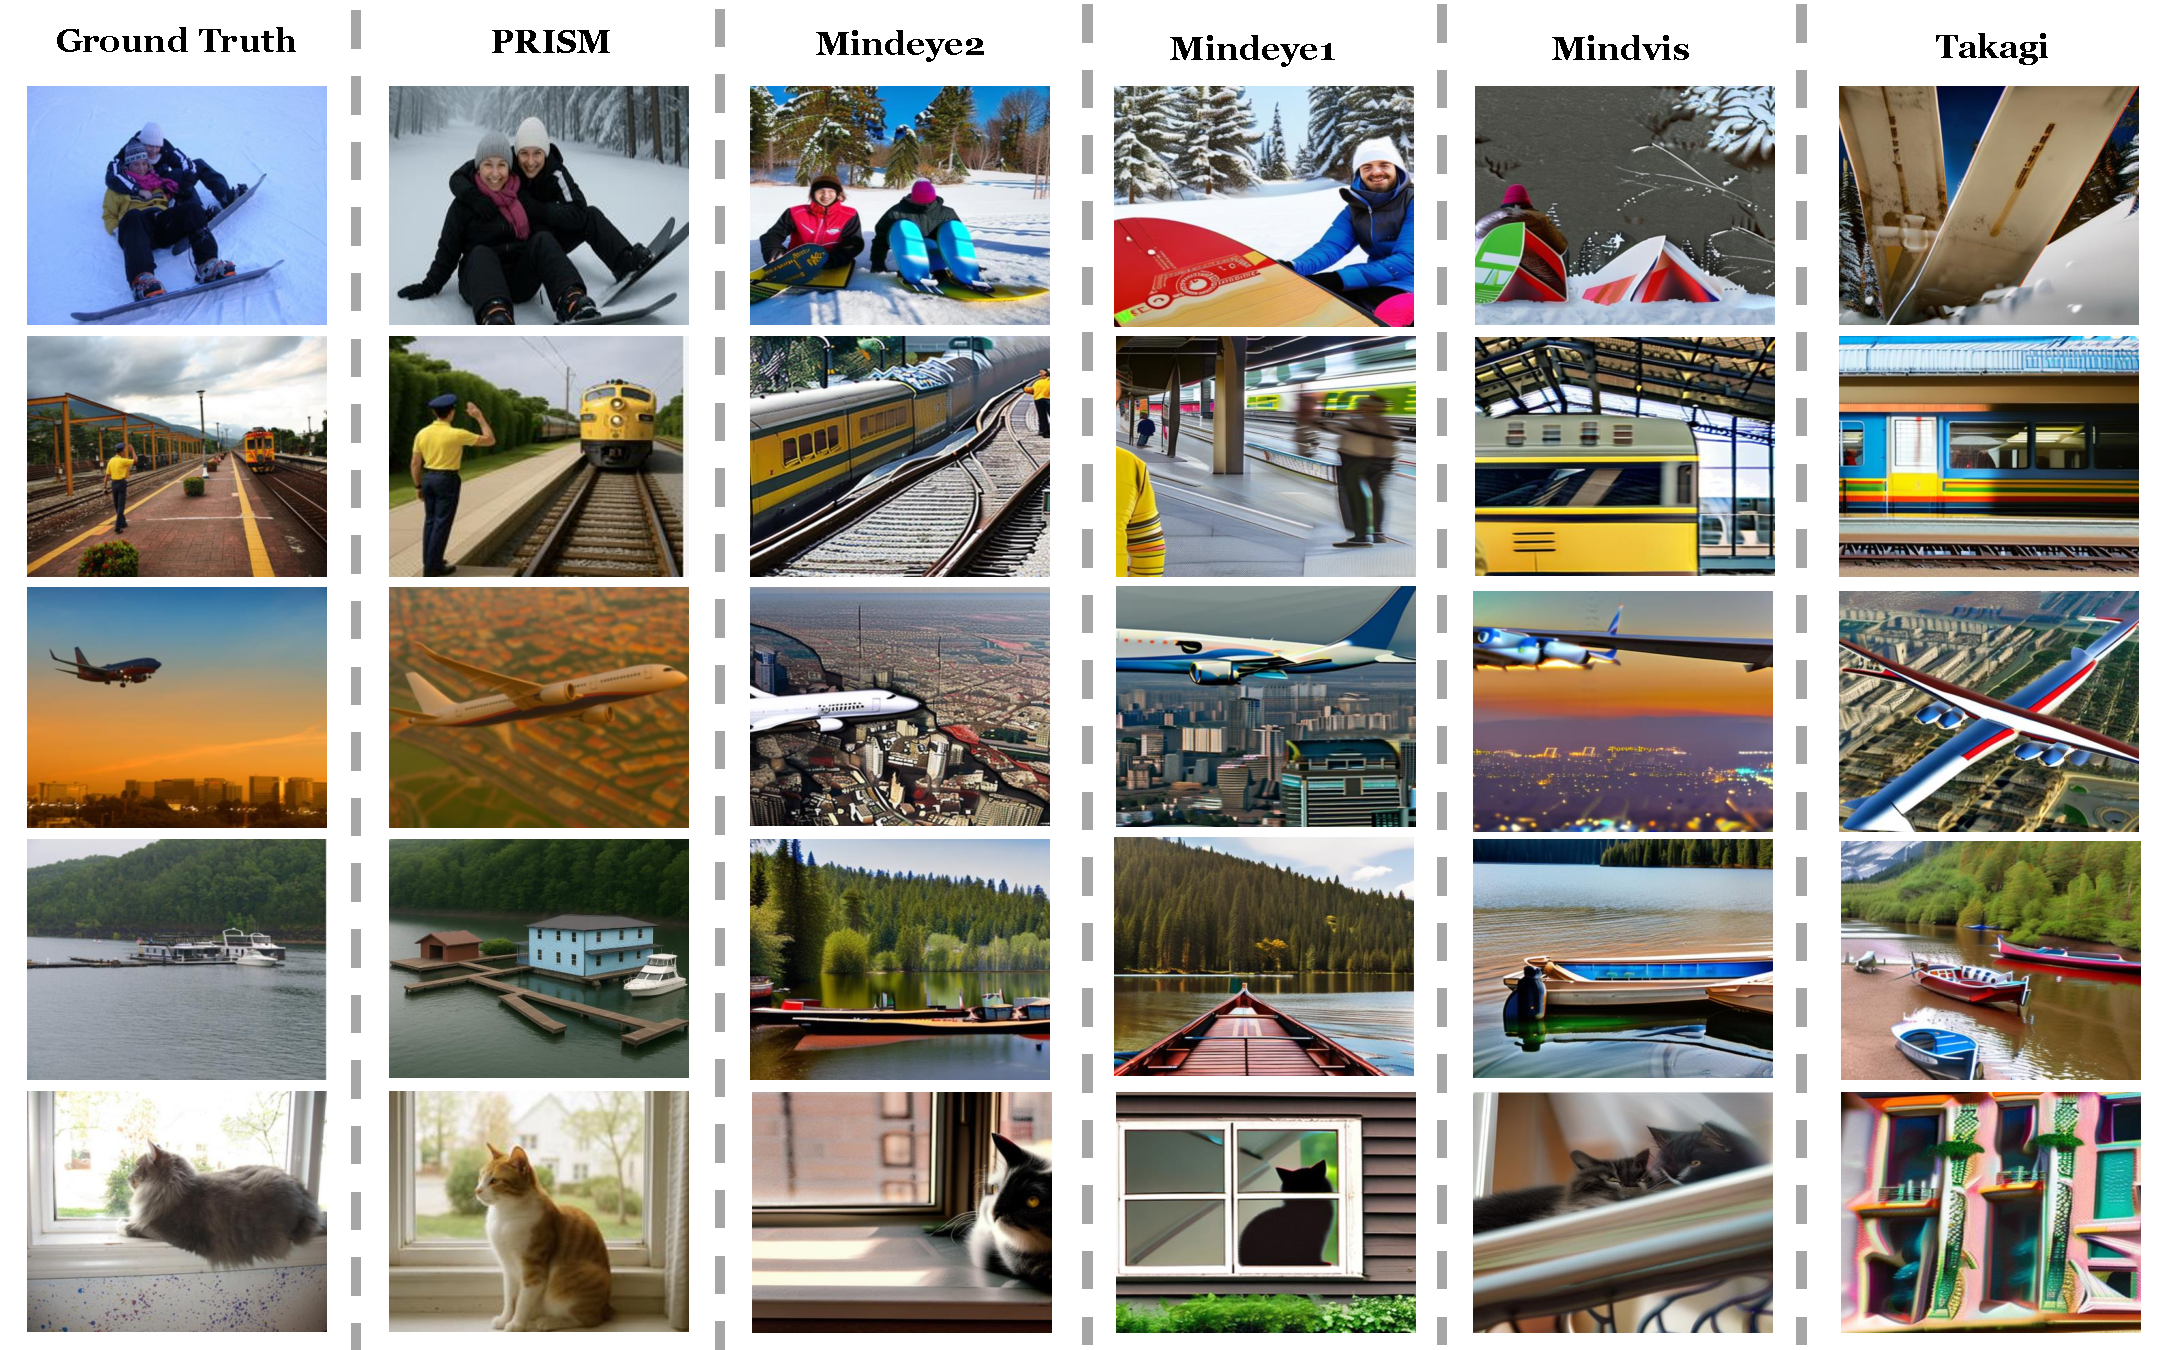
\includegraphics[width=0.9\linewidth]{figure/img_iclr.pdf}
    \vspace{-0.3cm}
    \caption{\small Reconstructed images from different methods. The first column shows the original viewed images. The rest of the columns show the reconstructed images from different methods. }
    \label{fig:reconstructed}
\end{figure}



We evaluate our fMRI-to-image reconstruction framework on test data and compare it with state-of-the-art methods.

\begin{table}   
\centering
\caption{\small Image QA results on reconstructed NSD images. \textbf{Mdvs}, \textbf{Mde1} and \textbf{Mde2} refer to \textbf{Mindvis}, \textbf{Mindeye1} and \textbf{Mindeye2}, respectively. Results are reported as accuracy, with the best highlighted in \textcolor{red}{red}.}
    % \resizebox{0.9\linewidth}{!}{

\begin{tabular}{lccccc}
\toprule

    & \textbf{\prism}   & \textbf{Takagi} & \textbf{Mdvs} & \textbf{Mde1} & \textbf{Mde2} \\
\midrule    
\textbf{Acc.}$\uparrow$ & \textcolor{red}{0.6054} & 0.4011    & 0.5037  & 0.5516   & 0.5765  \\
\bottomrule
\end{tabular}
% }
\label{tb:qa}
\end{table}




 Table \ref{tb:main} summarizes the results, with all metrics and standard deviations averaged across subjects over five runs. Visualizations of reconstructed examples from the test set are shown in Figure~\ref{fig:reconstructed}. As shown in Table \ref{tb:main}, \prism outperforms state-of-the-art methods across all datasets and metrics, with up to a 6\% improvement in LPIPS, indicating higher perceptual similarity to the original images. Unlike baselines such as Mindeye2~\citep{scotti2024mindeye2} and Mindeye1~\citep{scotti2023reconstructing}, which often ignore key objects, \prism successfully reconstructs all objects, yielding notable gains across all metrics. These results demonstrate the effectiveness of our framework in translating brain activity into accurate, perceptually aligned image reconstructions.
%The substantial improvements further highlight that our approach generates images that are not only structurally accurate but also perceptually closer to the original images, emphasizing the advantages of object-centric fMRI mapping and object diffusion in enhancing reconstruction quality. 





We further evaluate our method on a question answering (QA) task using reconstructed test images from the NSD dataset. For each image, we retrieve a corresponding question–answer pair from the COCO dataset~\citep{lin2014microsoft} and use Qwen2.5~\citep{bai2025qwen2} to answer the question based on the generated image. QA accuracy is reported in Table~\ref{tb:qa}. Our method achieves an accuracy of 60.54\%, significantly outperforming state-of-the-art methods. This demonstrates that our reconstructions are not only visually faithful but also semantically meaningful.







% We further conduct image question \& answering task on the reconstructed images on NSD dataset with Qwen2.5 \citep{bai2025qwen2}. The results are measured by the accuracy of getting the correct answer. The results are shown in Table \ref{tb:qa}. Our method achieves 60.54\% accuracy, outperforming the state-of-the-art methods by a large margin. This indicates that our method is capable of reconstructing images that are not only visually similar to the original images but also semantically meaningful.






\subsection{Ablation Study}

In this subsection, we present ablation studies to justify our choice of text as the latent space and to evaluate the effectiveness of the object-centric diffusion and attribute/relationship search modules.
% evaluate \prism's performance across different embedding variants and the contribution of each component in our framework to fMRI-to-image reconstruction performance. 
Experiments are conducted on the NSD dataset, though the trend generalizes to other datasets. 

\begin{table}{r}
\centering
\caption{\small Reconstruction performance across three latent spaces. The best result in each column is highlighted in \textcolor{red}{red}. $\uparrow$ indicates higher is better and $\downarrow$ indicates lower is better.}
\vspace{0.1cm}
% \resizebox{0.6\textwidth}{!}{
\begin{tabular}{lccccc}
\toprule
          
    \textbf{\small NSD}      & \textbf{PixCorr} $\uparrow$ & \textbf{SSIM} $\uparrow$  & \textbf{LPIPS} $\downarrow$  & \textbf{CLIP} $\uparrow$  & \textbf{Inception V3} $\uparrow$  \\ 

          %\multicolumn{5}{l}{\textbf{\small NSD}} &   \\
\midrule
\textbf{\prism}      & \textcolor{red}{0.3404$_{\pm 0.05}$}  & \textcolor{red}{0.4640$_{\pm 0.02}$}  & \textcolor{red}{0.5963$_{\pm 0.02}$} &     \textcolor{red}{0.9467$_{\pm 0.03}$}   & \textcolor{red}{0.9516$_{\pm 0.03}$}  \\
\textbf{Clip text} & 0.3208$_{\pm 0.04}$    & 0.3725$_{\pm 0.06}$ & 0.6611$_{\pm 0.05}$ &0.9197$_{\pm 0.02}$  &  0.9011$_{\pm 0.04}$  \\
\textbf{LDM}   & 0.2090$_{\pm 0.07}$  & 0.3727$_{\pm 0.07}$ & 0.7502$_{\pm 0.04}$ & 0.8602 $_{\pm 0.06}$ & 0.8925 $_{\pm 0.05}$ \\
\bottomrule
\end{tabular}
\label{tb:abl_diff_space}
% }
\end{table}



We first compare reconstruction performance across three latent spaces: (1) language model embeddings (ours), (2) CLIP text embeddings (CLIP-Text), and (3) the image latent space of a diffusion model (LDM). As shown in Table~\ref{tb:abl_diff_space}, aligning fMRI signals to the language model text space consistently outperforms the other two spaces across all metrics. This demonstrates that textual representations alone can capture multiple levels of visual information, making text space a more brain-aligned and effective intermediate representation for fMRI-to-image reconstruction. Results for the remaining two datasets are provided in Table~\ref{tb:app_abl_space} of the Appendix. 



\begin{table}{r} 
\vspace{-0.7cm}
    \centering
    \caption{\small Effectiveness of the object-centric diffusion module and attribute/relationship search module on NSD data. The best result is highlighted in \textcolor{red}{red}.}
% \resizebox{0.8\linewidth}{!}{
\begin{tabular}{lccc}
\toprule

               & \textbf{PixCorr} $\uparrow$ & \textbf{SSIM} $\uparrow$  & \textbf{LPIPS} $\downarrow$ \\
\midrule

\textbf{\prism}         & \textcolor{red}{0.3404$_{\pm 0.05}$}  & \textcolor{red}{0.4640$_{\pm 0.02}$}  & \textcolor{red}{0.5963$_{\pm 0.05}$} \\
\textbf{w/o ObjC.}     & 0.3291 $_{\pm 0.06}$  & 0.4299 $_{\pm 0.06}$ & 0.6111 $_{\pm 0.05}$ \\
\textbf{w/o AttOpt.+Bst}   & 0.3311$_{\pm 0.04}$    & 0.4421$_{\pm 0.01}$ & 0.6005$_{\pm 0.02}$ \\
%-t5+llama 2 7b & 0.3011  & 0.4094 & 0.6606\\
% -prompt opt + random select &     &  & \\ 
\textbf{w/o AttOpt.+Wst} &  0.3068 $_{\pm 0.05}$    & 0.4167$_{\pm 0.02}$  & 0.6398$_{\pm 0.05}$  \\ 

\bottomrule
\end{tabular}
% }
\label{tab:ablation}
\end{table}





Next, we evaluate the effectiveness of the two proposed modules. Results are in Table~\ref{tab:ablation}. To evaluate the Object-centric Diffusion module, we compare against a variant (\textbf{w/o ObjC.}) that replaces object-level cross-attention with standard U-Net cross-attention. To assess the attribute/relationship search module, we test two variants that skip the search process and rely only on the initial keyword set: \textbf{w/o AttOpt.+Bst}, which fixes the prompt to the highest-scoring (best) keyword, and \textbf{w/o AttOpt.+Wst}, which fixes it to the lowest-scoring (worst) keyword.
%The initial keywords are provided in Appendix~\ref{app:attr_opt}.




Overall, removing or replacing the two modules consistently degrades performance across all metrics. Specifically, eliminating object cross-attention leads to notable declines that cannot be recovered through prompt optimization, highlighting its essential role in reconstructing perceptually accurate images. Likewise, bypassing prompt optimization and using the best or worst initial attribute also reduces performance, indicating that the initial attributes alone are insufficient and underscoring the importance of prompt optimization in our model. The ablation study on the number of objects in our framework is shown in~\Cref{app_mlp} of the Appendix.


\subsection{Keyword Search}
\textbf{Case Study.} To better understand the keywords selected by our attribute/relationship search module, Table~\ref{tab:search_words} presents the top-scoring keywords across different rounds of the $\varepsilon$-greedy search.
% In this subsection, we describe the experimental setup for our attribute/relationship search, which aims to identify the key attributes and relationships encoded by brain signals during visual processing.
% The optimization is conducted on the training data using an $\varepsilon$-greedy search strategy with $\varepsilon = 0.5$, allowing a balance between exploration and exploitation over 40 update rounds. At each search round, we prompt the VLM to generate two new relationship keywords based on eight words in the current keyword set. 
% The search is initialized with six widely-used keywords describing object relationships: Semantic Relation~\citep{johnson2015image}, Positional Relation~\citep{lu2016visual,haldekar2017identifying}, Functional Relation~\citep{zhu2015understanding}, Action Relation~\citep{lu2016visual}, Visual Attributive Relation~\citep{farhadi2009describing}, and Part–Whole Relation\citep{lu2016visual}. For each type, we use \texttt{GPT-4o} to generate four synonymous keywords, resulting in an initial pool of 24 candidate attributes. We adopt the scoring function $\mathcal{S}(\mathbf{Y}_1,\mathbf{Y}_2) = 1 - \text{LPIPS}(\mathbf{Y}_1,\mathbf{Y}_2)$ as defined in Equation~\ref{eq:opt_obj}.  The CKA threshold $\alpha$ is initialized to the minimum CKA score among the initial candidates. 
The results show that, despite extensive exploration, the top-scoring keywords consistently converge toward spatially oriented relationships such as \texttt{Spatial Layout} and \texttt{Relative Position}. This suggests that: (1) descriptions emphasizing spatial information are most effective for guiding the diffusion model to accurately reconstruct images, as indicated by their highest LPIPS scores; and (2) these keywords also align well with fMRI data, as their CKA scores are no lower than those of the initial keywords, in accordance with the search constraints. This result is consistent with prior neuro-scientific findings showing that neural representations in the brain are sensitive to spatial arrangements and relative positions of objects~\citep{zopf2018representing, graumann2022spatiotemporal}. Therefore,  we use \texttt{Spatial Layout} as the optimal keyword $a$ to generate structured descriptions for model training.
{Additional implementation details of the attribute/relationship search module can be found in Section~\ref{app:attr_opt} of the Appendix. To further demonstrate its robustness, we perform an experiment where all spatial-related keywords are deliberately excluded from the initial keyword set. The results, presented in Section~\ref{app:new_keyword_search} of the Appendix, show that the module is still able to identify the relevant spatial keywords, demonstrating the robustness and effectiveness of our search process.
}


{
\color{black}
\textbf{Neuroscientific Interpretation of the Optimal Keyword.} To explore why the optimal keyword \texttt{Spatial Layout} exhibits stronger alignment with fMRI signals, we conduct a gradient-based interpretability analysis to examine the neural correlations of different keyword types. Specifically, during inference on the test set, we identify predicted words associated with spatial relationships (e.g., directional terms) and functional attributes (e.g., actions or behaviors of objects), and compute the gradients of these tokens with respect to the input fMRI signals. Ideally, larger gradients indicate that specific voxel values within the fMRI contribute more strongly to predicting the given keyword, and are thus more relevant to that semantic category. By averaging these gradients across samples, we identify the ROIs that contribute most to each keyword category. For spatial relationships, we observe the strongest activation in the ROI 119 (HCP mmp1 atlas)~\citep{glasser2016multi}, which belongs to Presubiculum (PreS), a region linked to spatial memory~\citep{dalton2017pre, boecker2024hippocampal}. In contrast, for functional attributes, the Ventromedial Visual Area 1 (VMV1, ROI 153 of HCP mmp1 atlas) shows the highest activation. Additionally, we compute the mean voxel intensity within each ROI and find that PreS exhibited a higher mean activation (0.0080) compared to VMV1 (0.0028). These findings suggest that the fMRI contains stronger activation in spatially relevant regions such as PreS, which may explain the higher alignment observed for spatial keywords. Nonetheless, we acknowledge that further validation from the neuroscience community is needed.
}
